% status: 0
% chapter: TBD

\title{Location based crime data search and analysis with Spark UDF}


\author{Kadupitiya Kadupitige}
\orcid{1234-5678-9012}
\affiliation{%
	\institution{Indiana University}
	\streetaddress{Smith Research Center}
	\city{Bloomington} 
	\state{IN} 
	\postcode{47408}
}
\email{jasakadu@iu.edu}

\author{Gregor von Laszewski}
\affiliation{%
  \institution{Indiana University}
  \streetaddress{Smith Research Center}
  \city{Bloomington} 
  \state{IN} 
  \postcode{47408}
  \country{USA}}
\email{laszewski@gmail.com}


% The default list of authors is too long for headers}
\renewcommand{\shortauthors}{G. v. Laszewski}


\begin{abstract}
This paper provides a sample of a \LaTeX\ document which conforms,
somewhat loosely, to the formatting guidelines for
ACM SIG Proceedings.
\end{abstract}

\keywords{hid-sp18-409, Crime data analysis, MapReduce, Google Maps, 
spark UDFs}


\maketitle


\section{Introduction}

A crime is generally defined as an act punishable by law and is one of
the dangerous factors for any
country\cite{hid-sp18-409-agarwal2013crime}. It is impossible to find
a country with a crime- free society due to complex causes such as
poverty, parental neglect, low self-esteem, alcohol, drug abuse and
etc~\cite{hid-sp18-409-bharathi2014survey,
hid-sp18-409-kiani2015analysis}.  Inspired by the big data revolution,
the historical way of crime solving and prevention has greatly
influenced and improved by the help of state-of-the-art data analytic
tools and machine learning research. Law enforcement officers have
started involving more data analytic expertises to speedup the crime
solving process highlighting that, it is an interdisciplinary research
area.

According to Chicago Police Department, crime prevention is important
and much more difficult to handle than crime solving for law
enforcement agencies~\cite{hid-sp18-409-www-cpd}. Law enforcement
officers could identify crime prone areas or suspicious activities
even before a crime is committed with the aid of pattern recognition
and big data analysis~\cite{hid-sp18-409-nath2006crime,
hid-sp18-409-gera2014city}.  According to the Los Angeles Police
Department (LAPD) and Chicago Police Department (CPD), whenever a
crime was committed somewhere, more crimes are likely to be occurred
in a nearby area, and the patterns of those criminal activities could
be identified through big data analysis~\cite{hid-sp18-409-www-cpd,
hid-sp18-409-www-lapd}. However, crime prevention could be so much
effective if there is an easy way to check the crime prone areas so
that people could be aware the of crime prone areas.

As inspired by the requirement to raise the awareness of crime prone
areas, we implement a location based crime search website where people
can find crimes happened near a particular geographical location (in a
vicinity area with inserted radius) for a given address. For this
project, we have selected a dataset which includes the crime
information from 2001 to current date in Chicago
city~\cite{hid-sp18-409-www-data.gov}. We further analyze this crime
dataset using the crime type, incident location and timestamps to
identify the trends of crime types for a particular geographical
area. There are many applicational use for this kind of a project such
as a user trying to buy a new house, may like to do a background
search on criminal activities around the geographical area for safety
concerns and a user who would like to visit some place would love to
know the seasonal and time effect on the crime rate in that location
before booking a hotel.

The organization of this project report is as follows. In section II,
a literature review on existing crime data analyses and crime
reporting web services are presented. Section III provides a
methodology followed in this project while section IV elaborates the
results and discussion. A summary about the project paper is provided
in section V.

\section{Literature Review}
The recent research and development in crime data investigation area
could be broadly categorized into two categories; analysis of
criminology~\cite{hid-sp18-409-agarwal2013crime,
hid-sp18-409-bharathi2014survey, hid-sp18-409-kiani2015analysis,
hid-sp18-409-nath2006crime, hid-sp18-409-gera2014city} and
applicational development of crime data visualization
platforms~\cite{hid-sp18-409-www-spotcrime,
hid-sp18-409-www-crimereports, hid-sp18-409-www-mylocalcrime,
hid-sp18-409-www-crimemapping}. Analysis of criminology data could be
further categorized into crime control and crime
suppression~\cite{hid-sp18-409-agarwal2013crime}. There exists many
research focused on analyzing crime data based on different
methodologies such as kmeans cluster
analysis~\cite{hid-sp18-409-gera2014city, hid-sp18-409-nath2006crime,
hid-sp18-409-agarwal2013crime}, time series
analysis~\cite{hid-sp18-409-wei2006time}, variational data mining
techniques~\cite{hid-sp18-409-chen2004crime}, geographical analysis
using using statistical techniques~\cite{hid-sp18-409-santos2016crime}
and etc. This study experiments combinations of these techniques to
build a crime data investigation platform and hence, they are
discussed in this section.

Agarwal et al.~\cite{hid-sp18-409-agarwal2013crime} have investigated
a comprehensive crime data analysis to identify the crime patterns and
predict crimes based on spatial data distribution of existing data
using kmeans clustering based approach and rapid miner tool. They have
only focused on homicide crime type and plotted the number of reported
crimes with respect to year for different clusters. This analysis had
helped them to conclude that homicide is decreasing from 1990 to 2011
in in England and Wales~\cite{hid-sp18-409-agarwal2013crime}.
Following Agarwal~\cite{hid-sp18-409-agarwal2013crime}, Kiani et
al.~\cite{hid-sp18-409-kiani2015analysis} have also studied the same
dataset to improve the clustering approach by assigning weights to the
features in the dataset and using Genetic Algorithm (GA) to optimize
the Outlier Detection using the same rapid miner tool. Gera et
al.~\cite{hid-sp18-409-gera2014city} have studied the possibility of
profiling the crimes using cluster analysis. Gera et
al.~\cite{hid-sp18-409-gera2014city} have analyzed all type of crimes
happened in Delhi police commission as well as through National Crime
Records Bureau (NCRB), Delhi, India. They have created a crime
database by interviewing concerned officers, through semi-structured
interviews, group discussion, participant observation, documentation
analysis and questionnaires in Delhi region to perform two types of
crime profiling based on types of crimes and types of areas. Finally
an association between two profiling methods were identified using
weka data mining tool. Similarly, Nath et
al.~\cite{hid-sp18-409-nath2006crime} also applied several clustering
algorithms to identify the association in crime data taken from
sheriff’s office in the city of New Orleans. They have also used a
semi-supervised learning technique for knowledge discovery from the
crime records and to help increase the predictive accuracy in the
crime data classification task.

Extensive time series analysis on Philadelphia crime data has been
studied by Wei et al.~\cite{hid-sp18-409-wei2006time}. They have
compared stationary and non stationary models, nonseasonal and
seasonal models, intervention and outlier models, transfer function
models, regression time series models, vector time series models, and
their applications using the crime data. They have further elaborated
the procedures of time series analysis including parameter estimation,
diagnostic checks, forecasting, and inference using autoregressive
conditional heteroscedasticity model and generalized autoregressive
conditional heteroscedasticity model~\cite{hid-sp18-409-wei2006time}.

Recent research done by DnzzL et al.~\cite{hid-sp18-409-dnzzl},
Abenassi et al.~\cite{hid-sp18-409-abenassi}, Agsarthak et
al.~\cite{hid-sp18-409-agsarthak} and Opencity et
al.~\cite{hid-sp18-409-open-city} have focused on investigation of
Chicago city crime dataset~\cite{hid-sp18-409-www-data.gov}.  DnzzL et
al.~\cite{hid-sp18-409-dnzzl} have compared the crime prediction
accuracies for logistic regression, multilayer perception and random
forest algorithms and reported the highest accuracy 86.5\% for
multilayer perception based methodology. Similarly, Agsarthak et
al.~\cite{hid-sp18-409-agsarthak} have also used the same dataset for
crime forecasting in Chicago city using machine learning Rest API
provided by Microsoft Azure. They had also performed a statistical
analysis and time series analysis on the crime
data~\cite{hid-sp18-409-agsarthak}. Abenassi et
al.~\cite{hid-sp18-409-abenassi} have implemented a web based software
to analyze the Chicago city crime data by primary type and the
time. Similarly, Opencity et al.~\cite{hid-sp18-409-open-city} have
also implemented a web interface to analyze the crimes with year,
wards, type and district. All these research and development had only
focused on analyzing the dataset but have not implemented a user
friendly web interface where users could search crimes near a given
address and analyze the geographical location that they are actually
interested.

There are few web based platforms which allow user to find the crime
incidents near a particular address or GPS location such as
Spotcrime~\cite{hid-sp18-409-www-spotcrime},
Crimereports~\cite{hid-sp18-409-www-crimereports},
Mylocalcrime~\cite{hid-sp18-409-www-mylocalcrime} and
Crimemapping~\cite{hid-sp18-409-www-crimemapping}. All these web based
platforms only show geographical locations of the crimes and lacks
crime data analysis with time and other categories. Those also lacks
many important features such as variable radius search, address auto
complete, clustering and highlighting crime prone areas and
etc. However, these approaches could be enhanced up a great extend.
Due to these facts, this project tries to implement a location based
crime data search website which allows users to search crimes near a
given address and analyze the crime data in one single web interface.

\section{Methodology}
As described in the literature review, most of the research on crime
data investigation focused on analyzing crimes by type of the crimes,
time series information and geographical location. These techniques
could be extended to a great extent for our crime data framework. In
this section, we describe the data acquisition, data preprocessing,
technology usage and implementation details of individual modules
based on python implementation. 

\subsection{Data Acquisition}\label{dataset}
We have selected a dataset which includes the crime information from
2001 to current date in Chicago
city~\cite{hid-sp18-409-www-data.gov}. Dataset is created with the
reported incidents of crime (with the exception of murders where data
exists for each victim) that occurred in the City of Chicago from 2001
to present, without the most recent seven days. Data is extracted from
the Chicago Police Department's Citizen Law Enforcement Analysis and
Reporting system. In order to protect the privacy of crime victims,
addresses are shown at the block level only and specific locations are
not identified. Datasets size is 1.5 gigabytes with 22 columns and
over 6 Million rows. Attribute information about the dataset are as
follows:

\begin{description}
	\item[ID]: Unique identifier for the record.  \item[Case
	Number]: The Chicago Police Department record
	Number.
        \item[Date]: Date when the incident
	occurred.
        \item[Date]: The partially redacted address where
	the incident occurred.
        \item[IUCR]: The Illinois Unifrom
	Crime Reporting code.
        \item[Primary Type]: The primary
	description of the IUCR code.
        \item[Description]: The
	secondary description of the IUCR code.
        \item[Location
	Description]: Description of the location where the incident
	occurred.
        \item[Arrest]: Indicates whether an arrest was made
	or not.
        \item[Domestic]: Indicates whether the incident was
	domestic-related.
        \item[Beat]: Indicates the beat where the
	incident occurred.
        \item[District]: Indicates the police
	district where the incident occurred.
        \item[Ward]: The ward
	where the incident occurred.
        \item[Community Area]: Indicates
	the community area where the incident occurred.
        \item[FBI
	Code]: Indicates the crime classification as outlined in the
	FBI.
        \item[X Coordinate]: The x coordinate of the location
	where the incident occurred. This location is shifted from the
	actual location for partial redaction but falls on the same
	block.
        \item[Y Coordinate]: The y coordinate of the location
	where the incident occurred. This location also is shifted
	from the actual location for partial redaction but falls on
	the same block.
        \item[Year]: Year the incident
	occurred.
        \item[Updated On]: Date and time the record was
	last updated.
        \item[Latitude]: The latitude of the location
	where the incident occurred.
        \item[Longitude]: The longitude
	of the location where the incident occurred.
        \item[Location]:
	The location where the incident occurred in maps format.
\end{description}

\subsection{preprocessing}
When sweep over the rows in the dataset, we noted that many missing
values in some of the rows and columns. Hence before using the
dataset, it is imperative to treat the missing values. Our analysis
highly depends on the column such as ID, Case Number, Date, Primary
Type, Location Description, Arrest, Latitude and Longitude. So we have
neglected the data rows where we found null values in any of the
important columns. We used python programming environment and Pandas
data processing library to achieve this task. These functionalities
are built in to the data handling APIs in our framework and
automatically triggered when update the data files using provided data
source update swagger services.

\subsection{Technology Usage}
We used Python as the main programming language in this project and
few web technologies such as HTML, CSS, JQuery and Google maps java
script API are used for the front end development of the project. Full
description of programming environments and library packages which
used to implement the crime analyzing and visualization framework, are
shown in Table~\ref{tab:technology}.
\begin{table}[]
\centering
\caption{Technologies used in the project}\label{tab:technology}
\begin{tabular}{*{2}{c}}
\toprule
Technology                      & Version \\
\midrule
Python programming environment  & 3.6     \\
Flask                           & 0.12    \\
connexion                       & 1.1.15  \\
decorator                       & 4.2.1   \\
python-dateutil                 & 2.6.0   \\
setuptools                      & 21.0.0  \\
numpy                           & 1.14.0  \\
scipy                           & 0.18.1  \\
pandas                          & 0.20.3  \\
scikit-learn                    & 0.18    \\
pyspark                         & 2.1.1   \\
scikit-learn                    & 0.18    \\
java run time environment       & 8.16.1  \\
Apache Spark standalone version & 2.3.0   \\
Swagger codegen                 & 2.1.2   \\
HTML                            & 5       \\
CSS                             & -       \\
Java Script                     & -       \\
JQuery                          & -       \\
Google Maps Java script API     & -       \\
Dygraphs                        & -       \\
Docker                          & 1.13.1  \\
\bottomrule
\end{tabular}
\end{table}

\subsection{Overview of crime search framework}
Figure~\ref{fig:overview} shows the suggested framework for crime data
analysis and visualization.  As shown in the Figure~\ref{fig:overview}
there two main users in the system such as regular user and the admin
user. Regular user is only accessing the Flask web application (see
Section~\ref{flaskWebApp}) to see the crime data trends in entire
chichago city or in a specific area selected by the user with a
desired address and a radius. This is achieved through the micro
services defined in the swagger service explained in the
Section~\ref{swaggerService}. Admin user can trigger data source
update and spark map reduce with basic authentication as elaborated in
the Section~\ref{sparkModule}. Screen captures of the Flask web
application are shown in Figure~\ref{fig:screencapture}. The complete
framework is dockerized to run within a Docker container allowing easy
installation.

\begin{figure}[htb]
	\centering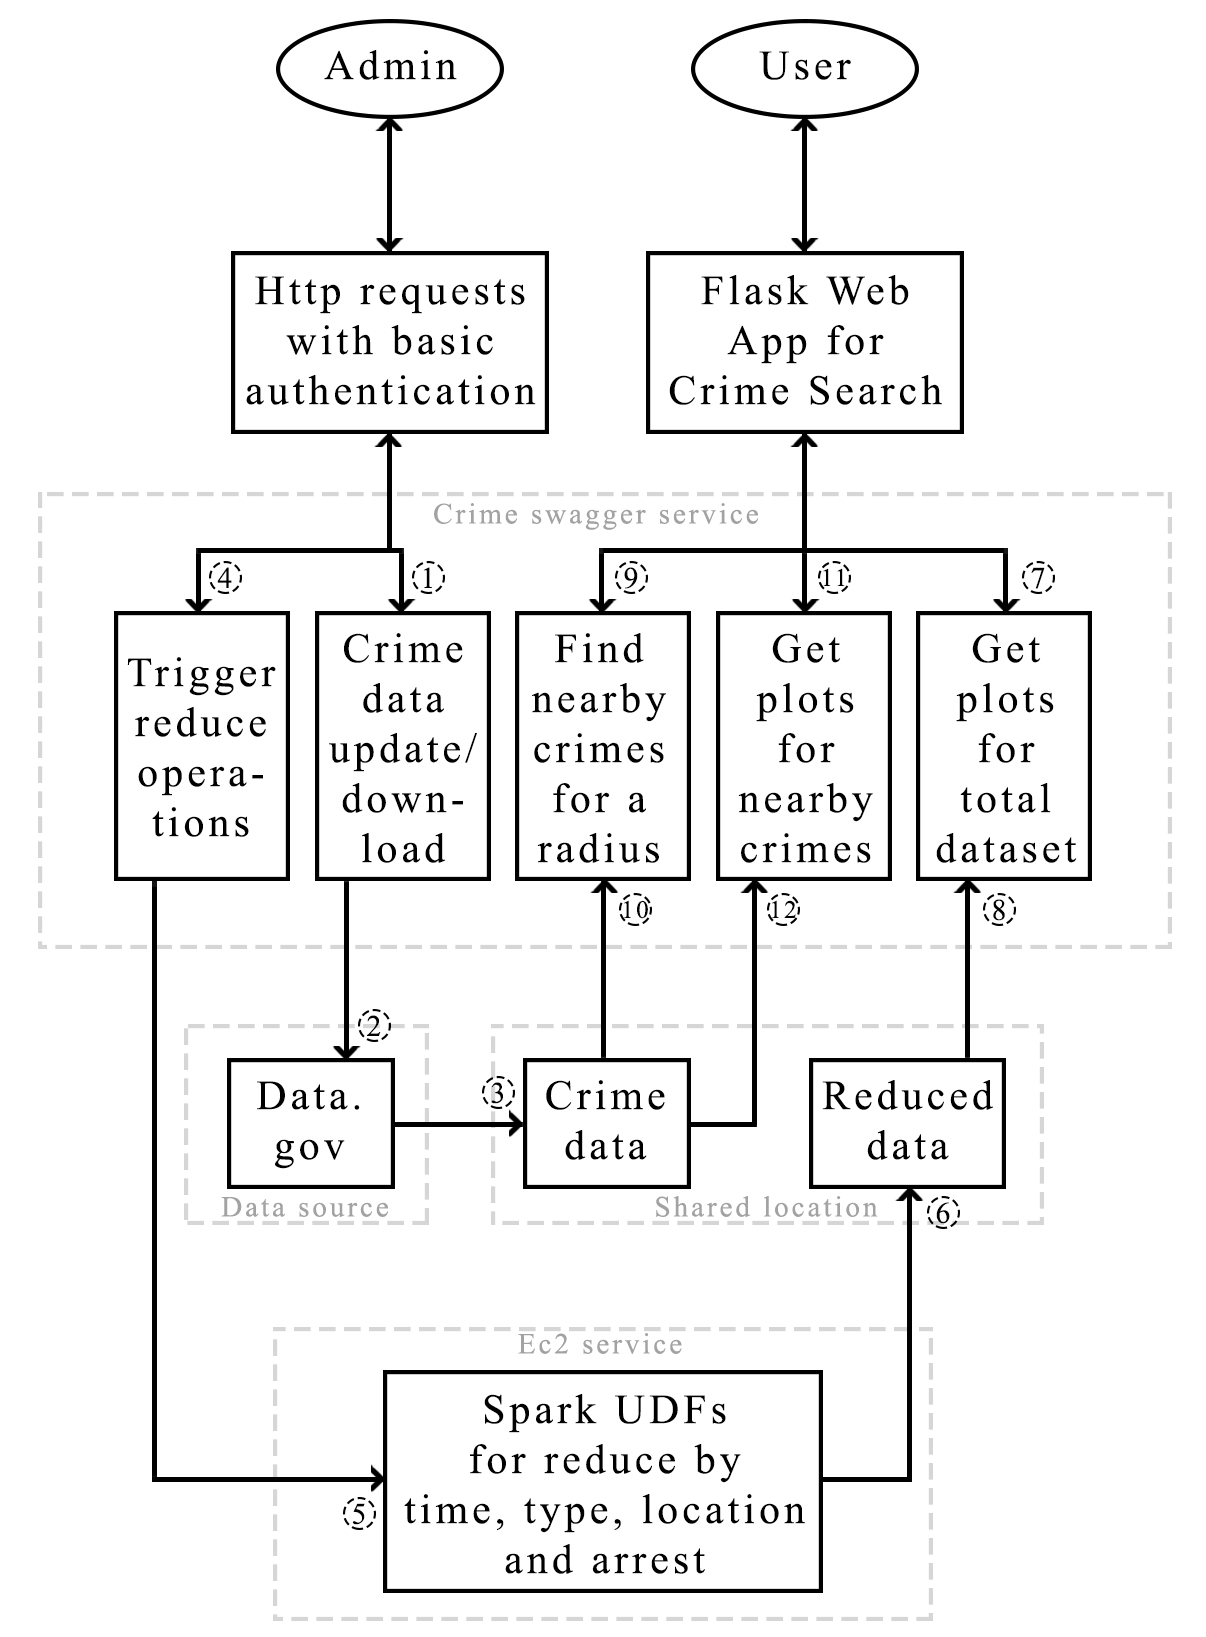
\includegraphics[width=\columnwidth]{images/overview.jpg}
	\caption{Overview
		of suggested framework for crime data
		analysis}\label{fig:overview}
\end{figure}

\begin{figure}[htb]
	\centering\includegraphics[width=\columnwidth]{images/flask-web-app-1.jpg}
	\caption{Screen captures of the Flask web application}\label{fig:screencapture}
\end{figure}

\subsection{Spark MapReduce module for crime analysis using time, type and location}\label{sparkModule}
Since the dataset described in Section~\ref{dataset} is so large to
handle in single core computer, we have implemented Spark MapReduce as
user defined functions (UDFs) for analyzing the dataset using time
series information, basic crime category and reported location of the
incident. These functionalities are only executed when the data source
is updated by the admin user. Following pseudocode explains how we
have implemented Spark MapReduce for the crime dataset.

\begin{verbatim}
1. Create a SparkSQL session
2. Load data with pandas
3. Process the data to get desired data columns
4. Create a Spark context with data
5. Create a RDD of Row objects using groups
6. Do the MapReduce based on the groups
\end{verbatim}

\subsection{Swagger web service for location based Crime analysis}\label{swaggerService}
As shown in Figure~\ref{fig:overview}, this swagger service contains
nine micro services to serve the Flask web application and admin
user. It also connect the admin user with Spark Mapreduce module and
stores the reduced data. As the dataset contained GPS coordinate for
every reported crime, we used famous Haversine formula to calculated
the distance between the users GPS location and the data points using
Equation~\ref{eq:haversine}
and~\ref{eq:haversine2}~\cite{hid-sp18-409-siahaan2017haversine}.

\begin{equation}\label{eq:haversine}
hav(\frac{d}{r}) = hav(\omega_2 - \omega_1) + \cos(\omega_1)\cos(\omega_2)hav(\lambda_2 - \lambda_1)
\end{equation}
\begin{equation}\label{eq:haversine2}
hav(\theta) = \sin^2(\frac{\theta}{2}) = \frac{1-\cos(\theta)}{2}
\end{equation}
Where:
\begin{description}
\item[$d$] is the radius of the sphere,
\item[$\omega_1$, $\omega_2$] are latitude of point 1 and latitude of point 2, in radians,
\item[$\lambda_1$, $\lambda_1$] are longitude of point 1 and longitude of point 2, in radians.
\end{description}
Following list contains the micro services defined and implemented inside the swagger service.

\begin{description}
	\item[getCrime]: User can search for a particular crime with
	unique crime Id using this API.
        \item[getCrimes]: The
	getCrimes API returns information about the crimes previously
	happened at a given location or nearby locations based on
	users GPS coordinates and radius. The response includes lists
	of crimes in the proper display
	order.
        \item[getFilteredCrimes]: This API endpoint returns
	information about the crimes previously happened at a given
	location or nearby locations based on user’s GPS coordinates,
	radius and a primary type (Example-
	BATTERY).
        \item[getPrimaryCrimeList]: User can get primary
	crime types as a list using this
	API.
        \item[getCrimesByMonth]: User can get top x number of
	crimes by month using this API.
        \item[getCrimesByYear]: User
	can get top x number of crimes by year using this
	API.
        \item[downloadData]: This API downloads the data from
	the data source difined in the config.yml
	file.
        \item[updateData]: This API updates the data from the
	data source difined in the config.yml
	file.
        \item[triggerSparkFuctions]: This API calls the Spark
	UDFs to generate the reduced data files for total crime
	dataset analysis.
\end{description}

\subsection{Flask web application for visualization}\label{flaskWebApp}
As illustrated in Figure~\ref{fig:overview}, Flask web application is
made for users to perform the crime data search based on their
geographical location and to visualize the crime data analysis by
utilizing the implemented swagger services described in
Section~\ref{swaggerService}. We have used Google maps javascript API
to showcase the crime data in correct geogrphical location. Following
sub sections describes the features of the developed web interface.

\subsubsection{Auto completed Addresses Search}\label{addressSearch}
We have used Google maps javascript address auto complete API to
provide a type-ahead search box for user to enter a address of any
location such as Establishment, Addresses and
Geocodes. Figure~\ref{fig:gui-addressSeach} shows the GUI widget which
we have created for this to achieve the address search. The radio
buttons allow users to filter the types of places that the
autocomplete returns. The Strict Bounds option restricts the search to
the area within the current viewport. If this option is not checked,
the API biases the search to the current viewport, but does not
restrict it.  When a user search this address it automatically creates a
marker on the Google map in the web interface. Inside this widget
functionality, we obtain the GPS coordinate for that particular
location and calls the ``getCrimes'' API described in
Section~\ref{swaggerService} to get the crime data points relevant to
the GPS coordinate and the radius entered inside the above mentioned
widget.

\begin{figure}[htb]
	\centering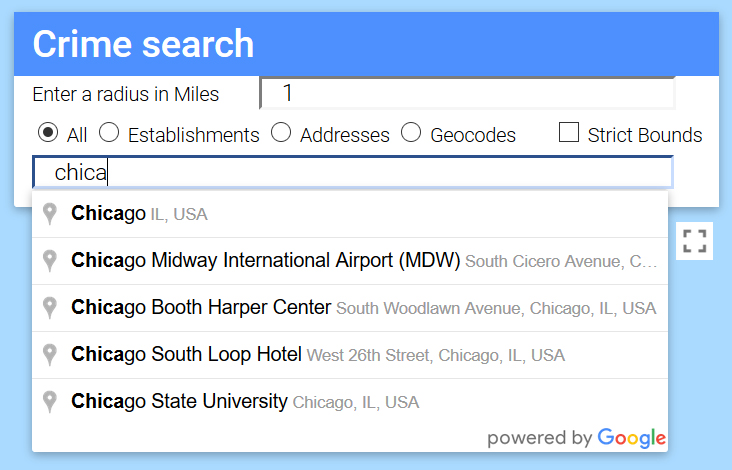
\includegraphics[width=\columnwidth]{images/addressSeach.jpg}
	\caption{Auto complete address search widget}\label{fig:gui-addressSeach}
\end{figure}

\subsubsection{Show crimes data in markers mode}\label{markerMode}
We have created a custom markers for each of the primary crime types
and kept those as templates to be used for creating markers for the
search results from the ``getCrimes'' API call described in
Section~\ref{addressSearch}. Bottom image in
Figure~\ref{fig:screencapture} shows how the markers are shown in
map. A legend about each of the crime types are put on the right
bottom pane as shown in Figure~\ref{fig:screencapture}. User can turn
on or off each of the crime types individually or group wise. When a
user click on a marker, a pop up window will appears as shown in top
right area of the Figure~\ref{fig:screencapture} and it contain
important information about that particular crime which was
clicked. We have also implemented some nice animation effects such as
markers bouncing, dropping and toggling to enhance the user experience
with the web interface. If needed user also can turn on or off all
markers using the functionality provided in the legend pane.

\subsubsection{Show crimes data in cluster mode}\label{clusterMode}
This cluster mode is created from the markers described in the
Section~\ref{markerMode} and there is a button placed on the legend
pane to activated the cluster mode and it automatically deactivate the
marker mode. This clustering mode is sensitive to the google maps zoom
level and it automatically reclusters based on the map zoom level. We
have achieved this using Google Marker Clusterer library which uses
the grid-based clustering technique that divides the map into squares
of a certain size (the size sensitive to the zoom level), and groups
the markers into each square grid. It creates a cluster at a
particular marker, and adds markers that are in its bounds to the
cluster. It repeats this process until all markers are allocated to
the closest grid-based marker clusters based on the map's zoom
level. The number on a cluster indicates how many markers it contains.

\subsubsection{Plots for crime data analysis}\label{plottingData}
There are two types of graphs created in the project such as graphs
which contains the information about entire crime dataset and graphs
which only contains the information about crime data a user searched
using a radius and an address as explained in
Section~\ref{addressSearch}. Both these types perform MapReduce
operation on the data considering time, type and location
information. The difference is that the graphs which requires
information about entire dataset, are plotted using the reduced data
from the Spark MapReduced module explained in the
Section~\ref{sparkModule}. These modes are enabled when user clicks on
button called ``Show Graphs'' in the bottom left of the web
interface. This button automatically changes to ``Hide Graphs'' and
shows the left pane (where graphs are plotted) shown in
Figure~\ref{fig:screencapture} as soon as user click on it. Immediate
plots demonstrate the plots for total crime by time, type and location
as shown in top left of the Figure~\ref{fig:screencapture}. User can
click on the ``Analyze Search Result'' button to see the top ten crime
trends near the location which was searched. These graphs were created
using the Dygraphs javascript library and contains many responsive
features such as drag on axis, zoom and unzoom, move along axis to
increase ability of the data visualization.

\section{Results and Discussion}
This section provides the results we have achieved through the
implemented crime data search and analyzing framework and provides a
discussion about the results. It contains the benchmarking results,
time series analysis results, geospatial analysis results and
statistical analysis results.

\subsection{Benchmarking}
We measured and analyzed the performance of the crime search framework
on three different hardware infrastructures as listed follows:
\begin{description}
	\item[Asuz Laptop]: 2 hardware cores, 2 threads per core, 8th
	Generation Intel Core i5-8300H processor (up to 3.9 GHz) with
	8 GB DDR4 high-frequency 2666 MHz RAM, 1 TB SSHD hard drive
	and GeForce GTX 1050 1GB VGA.
        \item[Dell Workstation]: 10
	hardware cores, 2 threads per core, Intel® Xeon® Processor
	E5-2630 V4 Family (up to 3.1 GHz) with 32 GB DDR4
	high-frequency 2133 MHz RAM, 500 GB SSD hard drive and NVIDIA
	Quadro M2000 4GB VGA.
        \item[EC2 EMR (m4.xlarge instances)]: 5
	nodes (1 master and 4 worker), 18 hardware cores per node, 2
	threads per core, Intel® Xeon® Processor E5-2686 v4 Family (up
	to 3.0 GHz) with 32 GB DDR4 high-frequency DDR4-2400 MHz RAM,
	with Spark 1.6 on Hadoop 2.6.0 YARN.
\end{description}

Since our frameworks takes an address and a radius value from the user
as explained in Section~\ref{addressSearch}, the data size for
MapReduce operation increases with the radius. So we measured time it
takes to perform the map reduce operations with different radius
(different data sizes) values on all three computing platforms
explained above. As our data set is from Chichago city area, we
increase the radius from 0.1 miles to 25 miles. The total execution
times (in minutes) for different data sizes (number of crimes) in
three different computing platforms are shown in the
Table~\ref{tab:performance}. We were able achieve a maximum speed up
of 32.5 with total 144 threads in EC2 m4.xlarge instances for the
complete dataset.

\begin{table}[]
	\centering
	\caption{Total execution times in minutes for different data sizes in different computing platforms}\label{tab:performance}
	\begin{tabular}{*{5}{c}}
		\toprule
		Radius & Data size &  laptop & workstation &  EC2 EMR \\
		\midrule
		0.1 & 52664  & 16  & 3 &  2 \\
		0.2 & 195334 & 23  & 5 &  2 \\
		0.4 & 444744 & 39  & 7 &  3 \\
		0.8 & 995512 & 68  & 12 &  3 \\
		1.6 & 1859480 & 102  & 19 &  3 \\
		3.2 & 3289296 & 172  & 32 &  5 \\
		6.4 & 5195988 &  307 & 58 &  10 \\
		12.8 & 6516889 & 364  & 72 &  12 \\
		25.6 & 6568036 & 391  & 75 &  12 \\

		\bottomrule
	\end{tabular}
\end{table}

\subsection{Time Series Analysis}

\begin{figure}[htb]
	\centering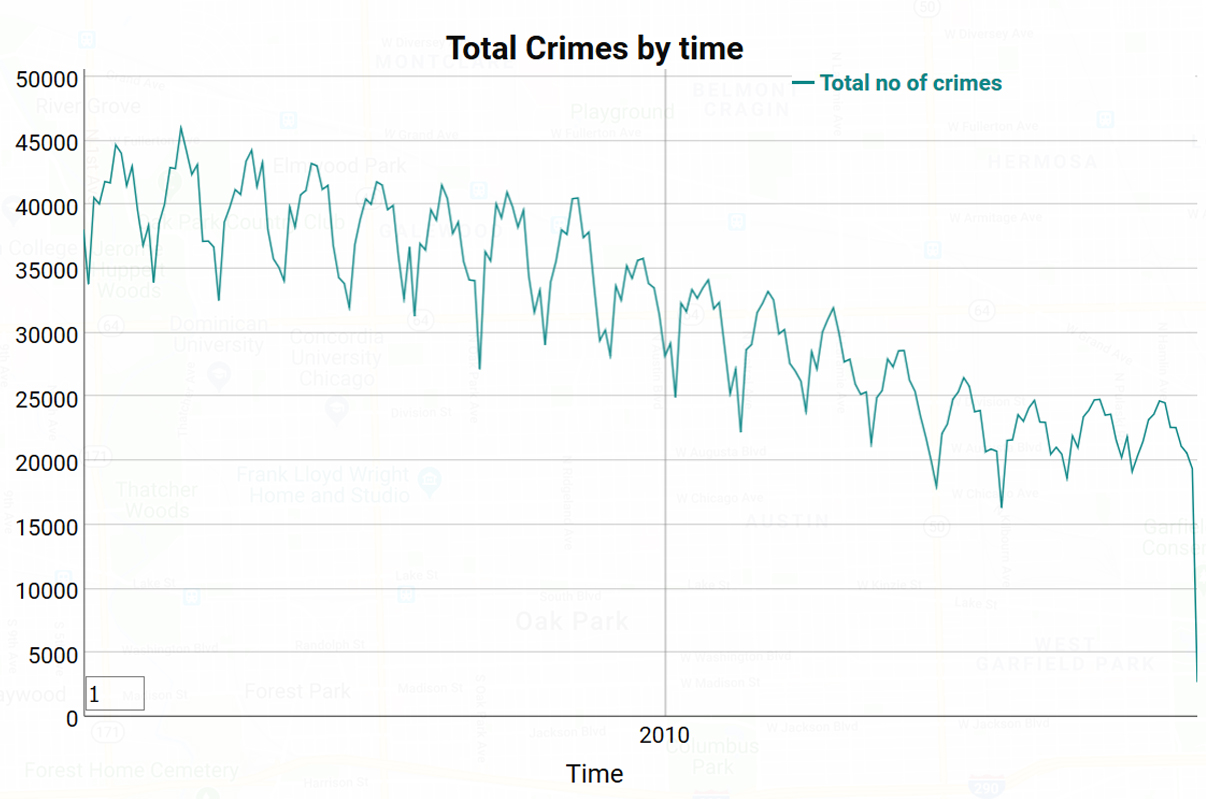
\includegraphics[width=\columnwidth]{images/time1.jpg}
	\caption{Total crimes for each month in Chichago from 2001-01 to 2018-02}\label{fig:time-totalCrime}
\end{figure}

\begin{figure}[htb]
	\centering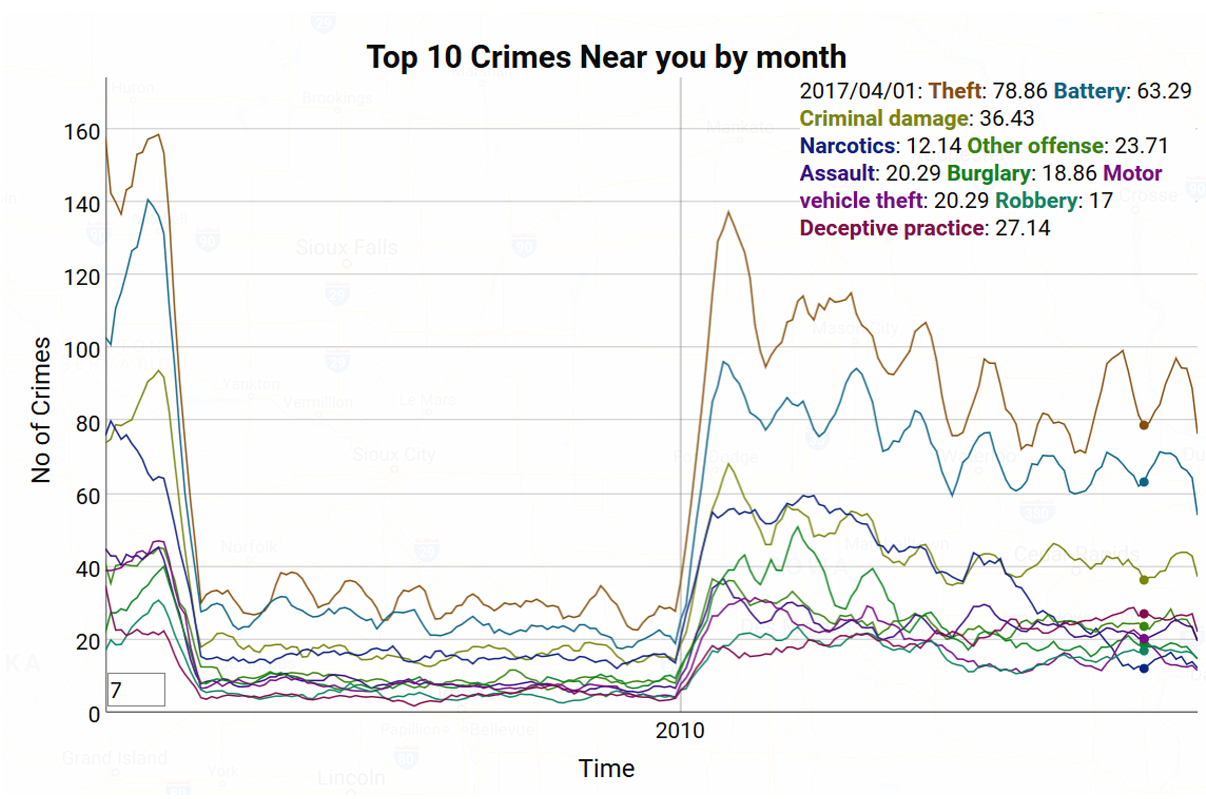
\includegraphics[width=\columnwidth]{images/time2.jpg}
	\caption{Most frequent crimes near (1.6 miles) Chichago Cook county for each month from 2001-01 to 2018-02 }\label{fig:time-top10crimes-local}
\end{figure}

\begin{figure}[htb]
	\centering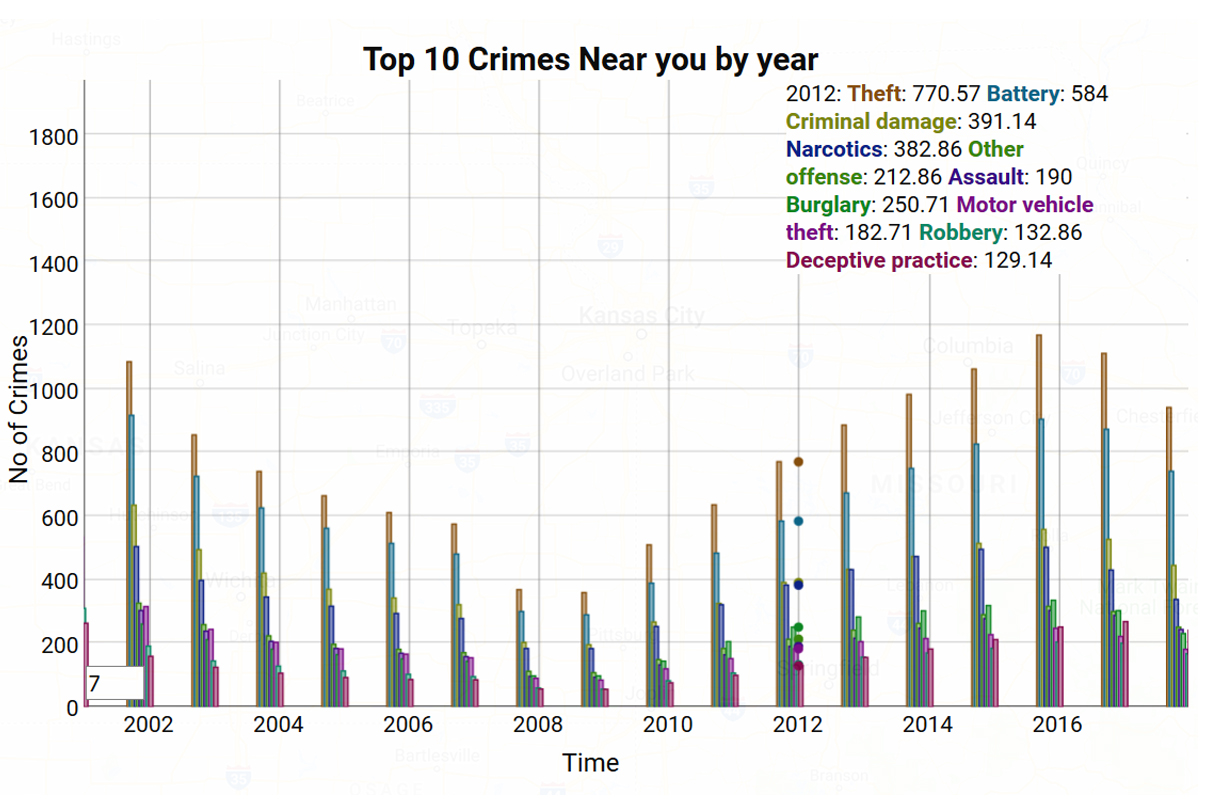
\includegraphics[width=\columnwidth]{images/time3.jpg}
	\caption{Most frequent crimes near (1.6 miles) Chichago Cook county for each year from 2001 to 2018}\label{fig:year-top10crimes-local}
\end{figure}


\subsection{Geospatial Analysis}

\begin{figure}[htb]
	\centering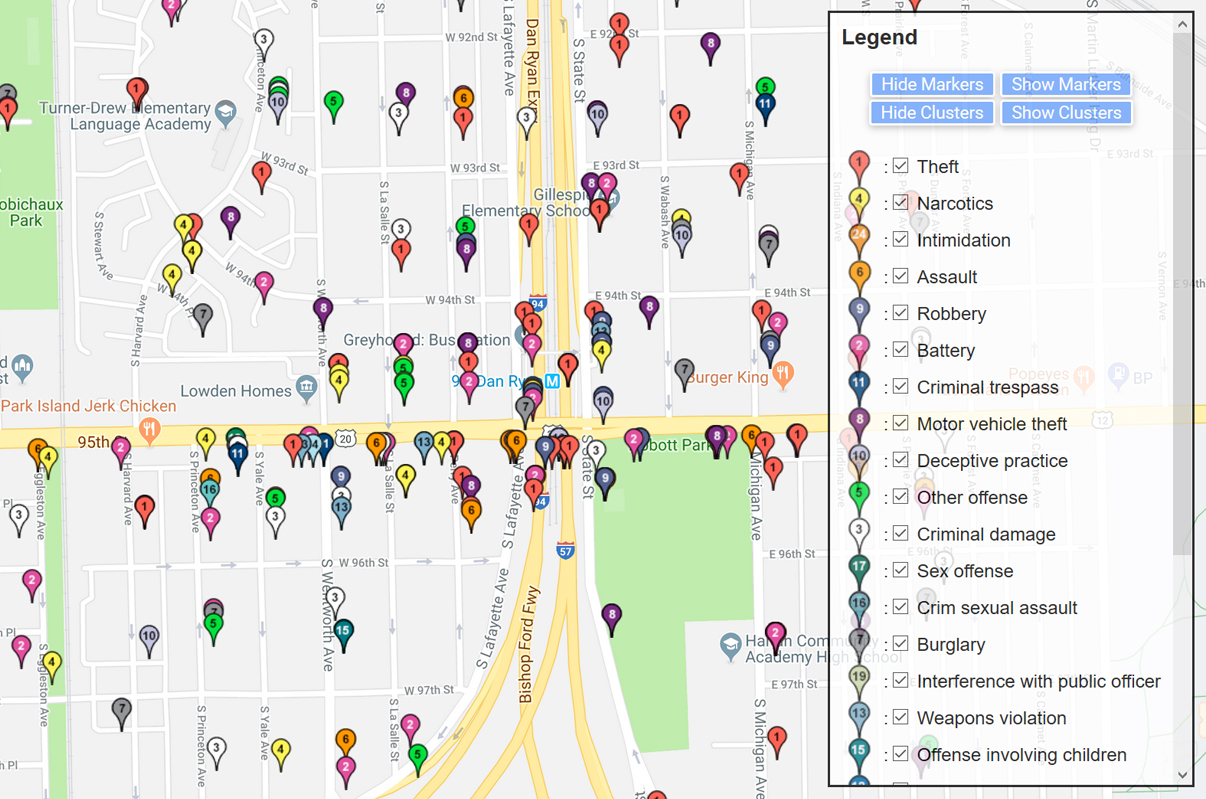
\includegraphics[width=\columnwidth]{images/geo1.jpg}
	\caption{Different types of crimes distribution on Google maps near (1.6 miles) Chichago Cook county}\label{fig:time-totalCrime}
\end{figure}

\begin{figure}[htb]
	\centering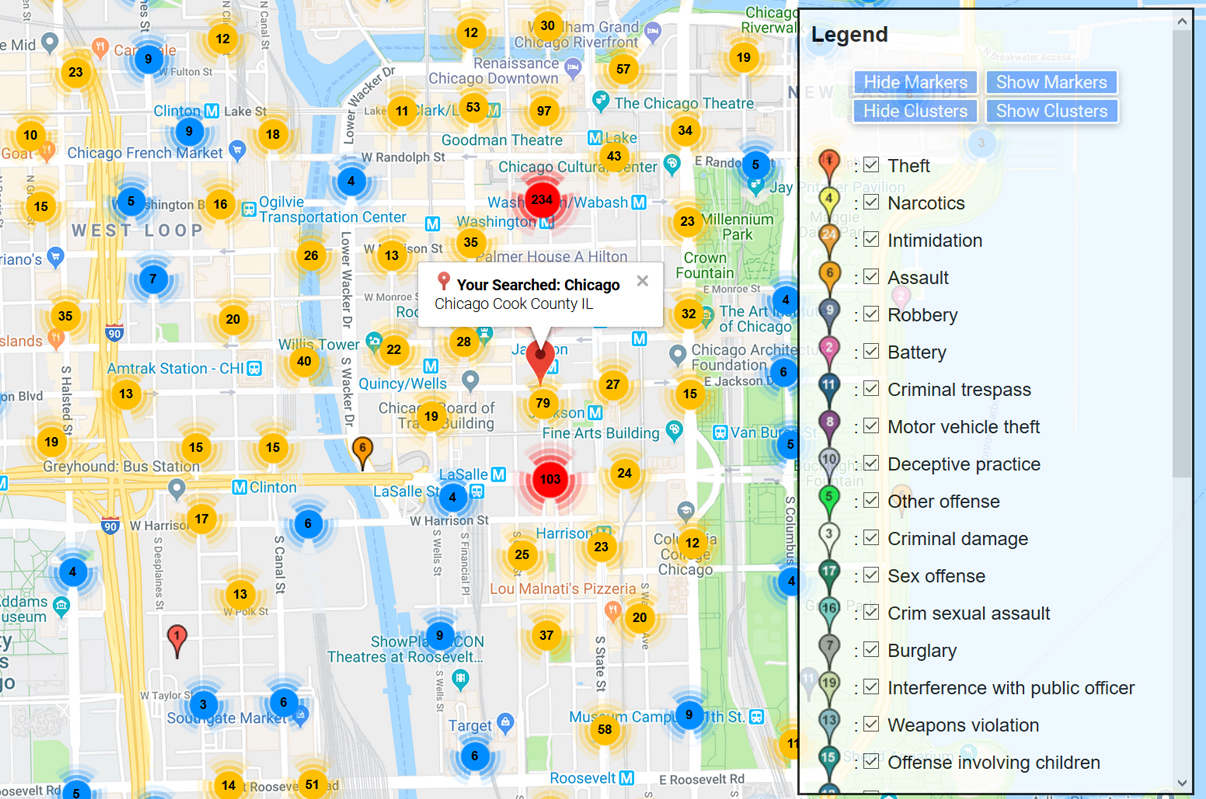
\includegraphics[width=\columnwidth]{images/geo2.jpg}
	\caption{Cluster mode for total crimes distribution on Google maps near (1.6 miles) Chichago Cook county}\label{fig:time-top10crimes-local}
\end{figure}

\begin{figure}[htb]
	\centering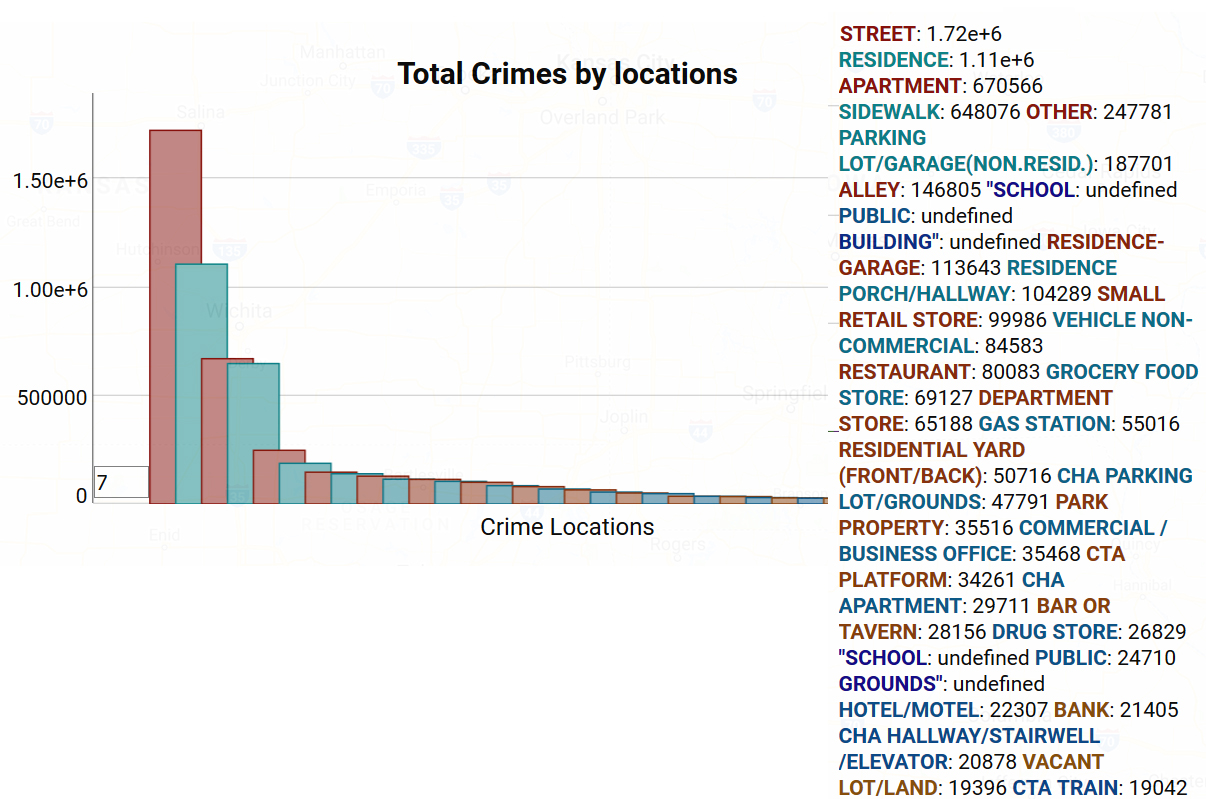
\includegraphics[width=\columnwidth]{images/geo3.jpg}
	\caption{Total Crimes by different locations in Chichago city from 2001 to 2018}\label{fig:year-top10crimes-local}
\end{figure}

\begin{figure}[htb]
	\centering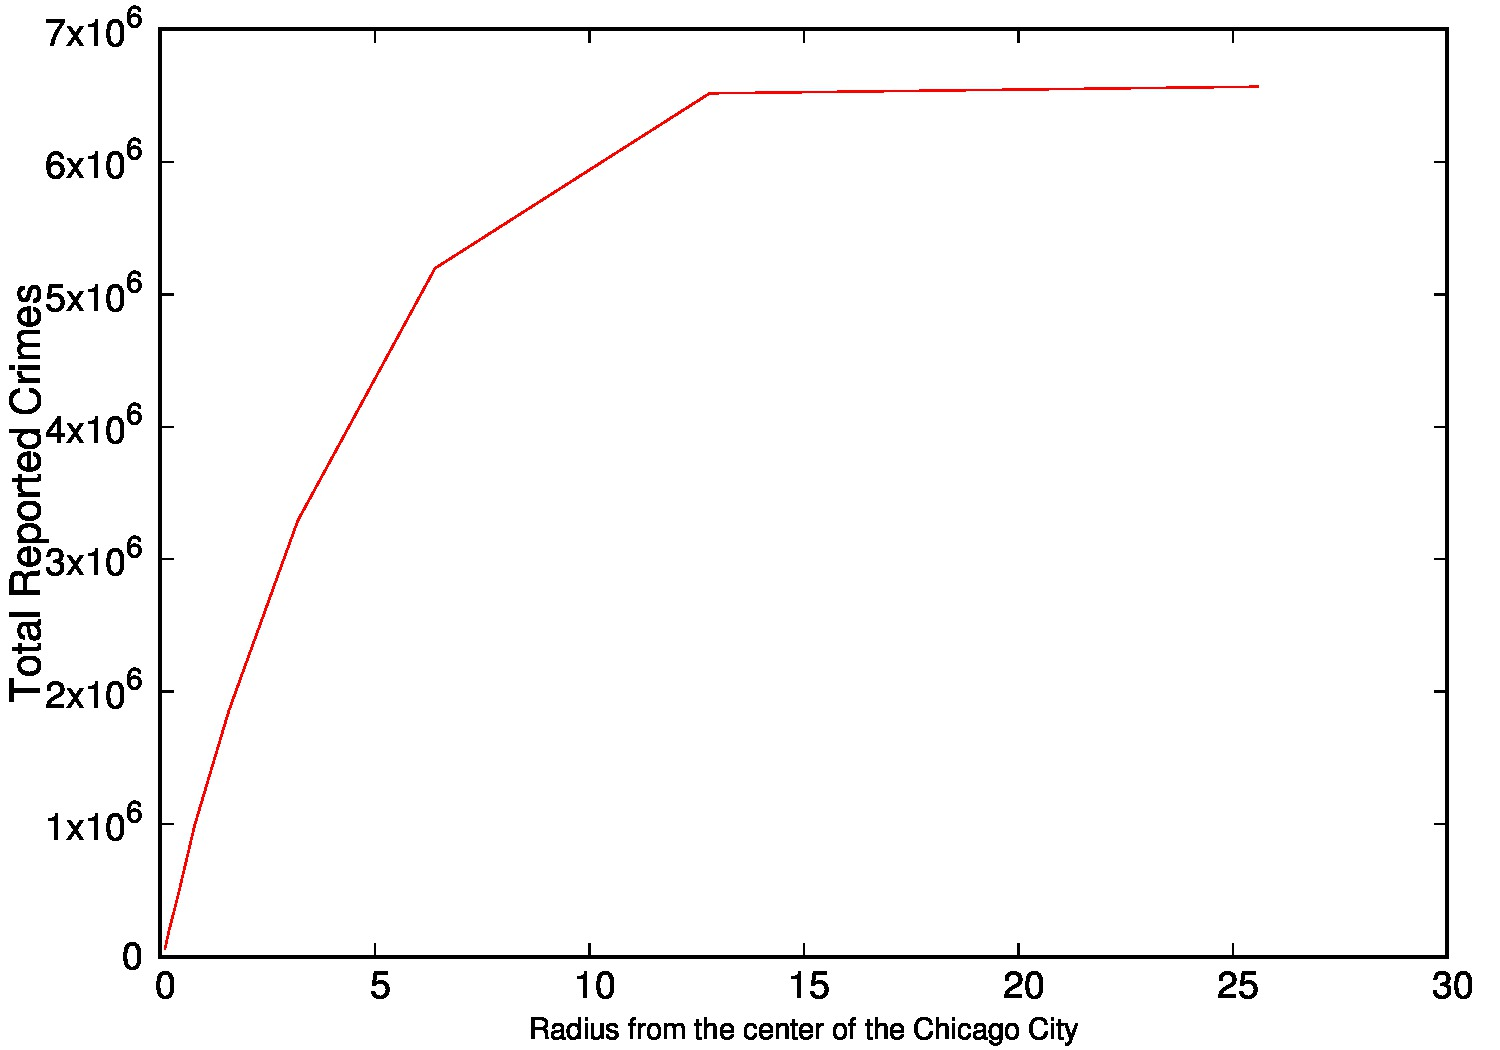
\includegraphics[width=\columnwidth]{images/geo4.jpg}
	\caption{Total Crimes by with increasing radius from the center of the Chichago city}\label{fig:crimes-with-radius}
\end{figure}

\subsection{Statistical Analysis}

\begin{figure}[htb]
	\centering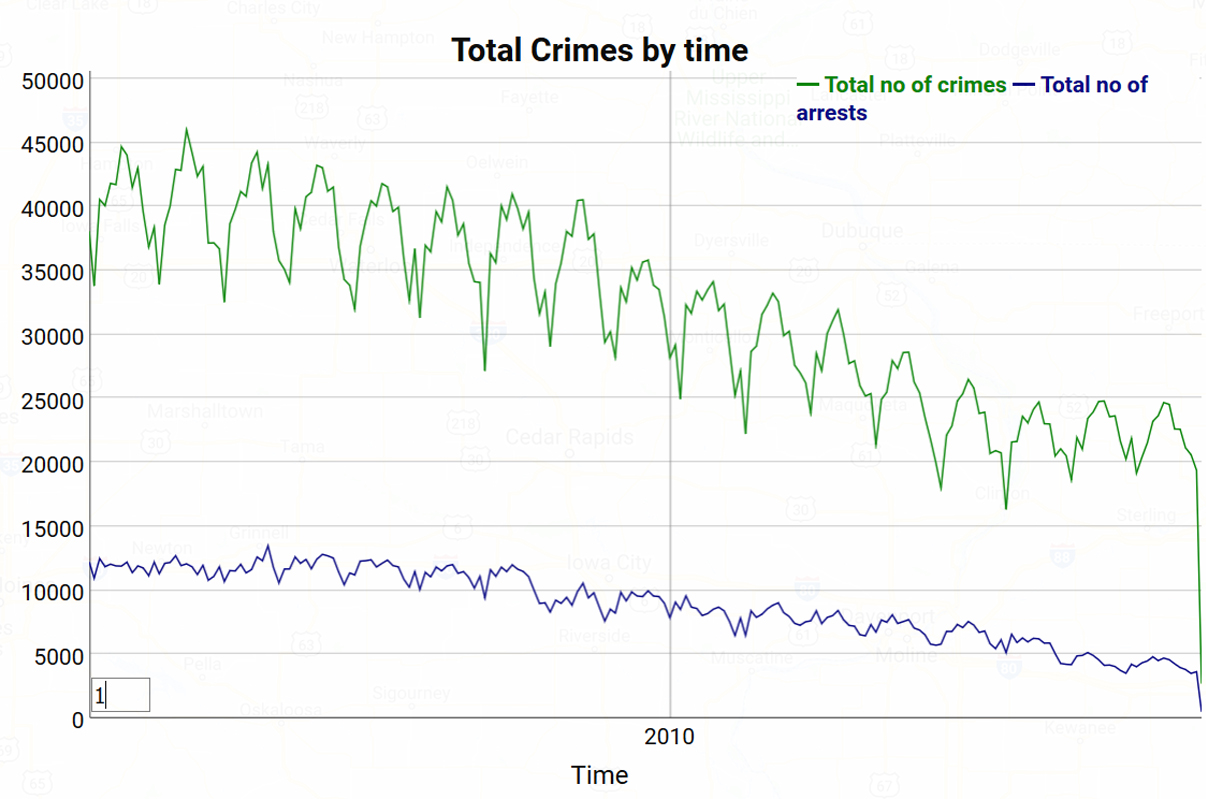
\includegraphics[width=\columnwidth]{images/stat1.jpg}
	\caption{Total crimes vss total arrests for each month in Chichago from 2001-01 to 2018-02}\label{fig:time-top10crimes-local}
\end{figure}

\begin{figure}[htb]
	\centering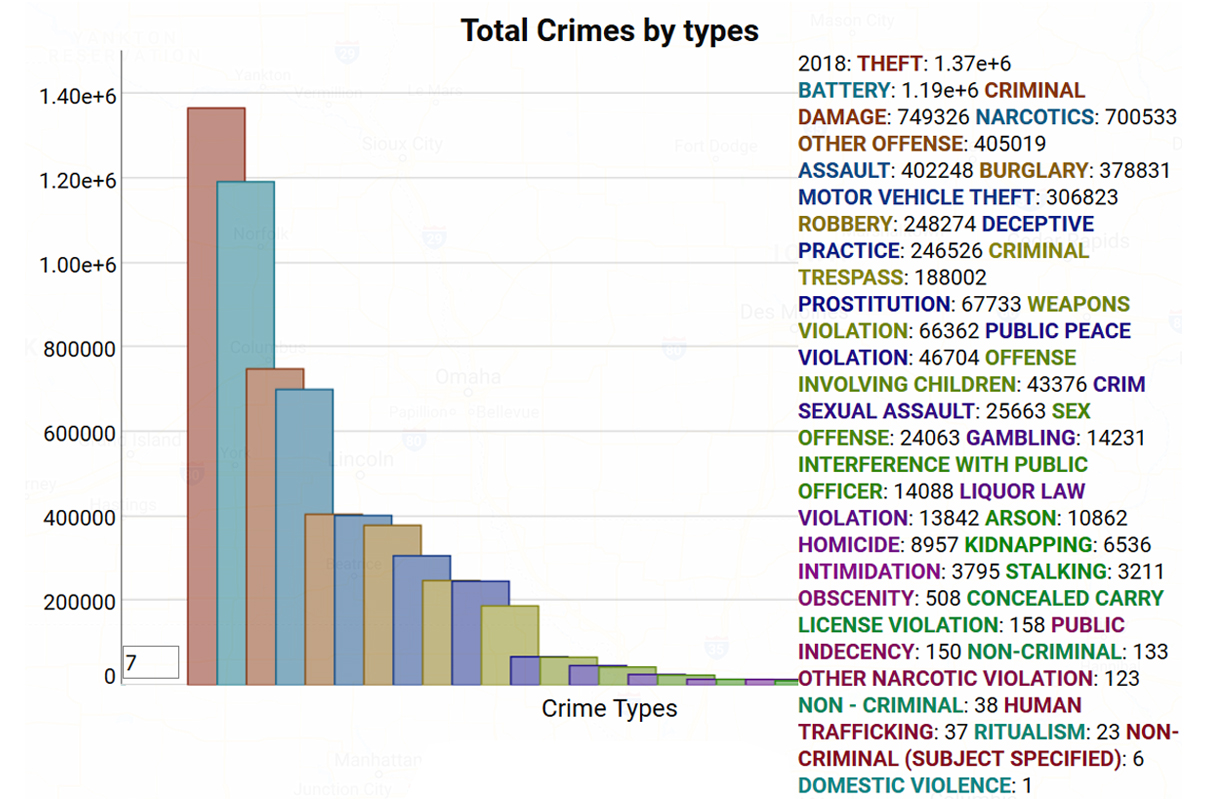
\includegraphics[width=\columnwidth]{images/stat2.jpg}
	\caption{Total Crimes by crime types in Chichago city from 2001 to 2018}\label{fig:year-top10crimes-local}
\end{figure}

\section{Conclusion} 

\begin{acks}
	
The authors would like to thank Dr.~Gregor~von~Laszewski for his
support and suggestions to write this extended abstract.
	
\end{acks}

\bibliographystyle{ACM-Reference-Format}
\bibliography{report} 